\renewcommand{\theHsection}{A\arabic{section}}


\begin{longtable}{ll}
        	{\bf Notation} & {\bf Description} \\
         \hline \\
         $[M]$ & $\{1, 2, \cdots, M\}$ for any positive integer $M$ \\
        $\bm{x}_{a:b}$ &  $(x_a,\ldots,x_b)$ for integers $a$ and $b$, $1\le a<b\le n$ \\
        $\tau_0$ & average instantaneous effect \\
        $\tau_j$ & average $j$-th period lagged effect \\
        $\bm{\tau}$ & $\begin{pmatrix} \tau_\ell & , & \cdots, & \tau_0   \end{pmatrix}$ \\
        $\*{y}_t$ & $\big(Y_{1t} , Y_{2t} , \cdots , Y_{Nt}\big)^\T \in \+R^{N \times 1}$\\
        $\*z_t$ & $\big(z_{1t} , z_{2t} , \cdots , z_{Nt}\big)^\T \in \{-1,1\}^{N \times 1}$\\
        $\bm{y}$ & $\big(
	\*y_1^\T , \*y_2^\T , \cdots , \*y_T^\T\big)^\T \in \+R^{NT\times 1}$\\
 $\bm{z}$ & $\big(\*z_1^\T , \*z_2^\T , \cdots , \*z_T^\T\big)^\T \in \+R^{NT\times 1}$ \\
 $Y$ & $\big(
	\*y_1 , \*y_2 , \cdots , \*y_T\big) \in \+R^{N\times T}$  \\ 
 $Z$ & $\big(
	\*z_1 , \*z_2 , \cdots , \*z_T\big) \in \{-1,1\}^{N\times T}$ \\
 $\omega_t$ & equals $N^\I \sum_{i = 1}^N z_{it}$ \\
 $\zeta_i$ & equals $T^\I \sum_{t = 1}^T z_{it}$ \\
 $A_i$ & first time that unit $i$ adopts the treatment, $A_i \in [T]  \cup \{\infty\}$ \\
 $A$ & $(A_1, \cdots, A_N^\T)$ \\
 $\alpha_i$ & unobserved unit fixed effect \\
 $\beta_t$ & unobserved time fixed effect \\
 $\*X_i$ & observed covariates of dimension $d_x$ \\
 $\*u_i$ & observed covariates of dimension $d_u$ \\
 $\bm{\theta}_t$ & unobserved coefficients of $\*X_i$ at time $t$ \\
 $\*u_t$ & unobserved coefficients of $\*v_t$ at time $t$ \\
 $\varepsilon_{it}$ & residual of unit $i$ at time $t$ \\
 $\sigma_\varepsilon^2$ & equals $\+E[\varepsilon^2_{it}]$ \\
 $\xi_\varepsilon^2$ & equals $\+E[(\varepsilon^2_{it} - \sigma_\varepsilon^2)^2]$ \\
 $e_{it}$ & equals $\varepsilon_{it} + \*u_i^\T \*v_t$ \\
 $\bm{1}_N$ & a vector of all ones of dimension $N$ \\
 $\*I_N$ & identity matrix of dimension $N \times N$\\
 $\hat{\tau}_j$ & estimate of $\tau_j$ \\
 $\hat{\bm{\tau}}$ & estimate of $\bm{\tau}$ \\
 $\xrightarrow{d}$ & convergence in distribution\\
 $\xrightarrow{p}$ & 
 convergence in probability \\
 \multicolumn{2}{l}{For a set of random variables $\tilde{X}_n$ and constants $a_n$,} \\
 $\tilde{X}_n = O_p(a_n)$ & the set of values $\tilde{X}_n/a_n$ is stochastically bounded \\ 
 $\tilde{X}_n = o_p(a_n)$ &  the set of values $\tilde{X}_n/a_n$ converges to zero in probability \\ 
 $A\mathrm{Cov}$ & asymptotic covariance\\
 \hline
 \caption{Mathematical notations.}
 \label{tab:notations}
    \end{longtable}


    \newpage

    \setcounter{tocdepth}{2}


    
    \tableofcontents

    \newpage
  
  \section{Supplementary Material for Non-Adaptive Experiments}\label{sec:constant-appendix}
		

		
		\subsection{Supplementary Material for Generalized Least Squares}\label{subsec:gls-carryover}
		
		    {\blue GLS estimates $\tau_0, \cdots, \tau_\ell$, $\alpha_i$, $\beta_t$, and $\bm{\theta}_t$ in \eqref{eqn:model-setup} by solving the following optimization problem } \begin{align} \label{eqn:gls}
        \min_{\bm{\tau}, \bm{\alpha}, \bm{\beta}_{(\ell+1):T}, \bm{\theta}_{(\ell+1):T} } \quad & \sum_{t=\ell+1}^{T} \bm{e}_t^\T   \cdot \*W^{-1} \cdot  \bm{e}_t   \\
       \nonumber \mathrm{s.t.} \quad & \bm{e}_t =  \*y_t - \bm{\alpha} - \beta_t \cdot \bm{1}_N  - \*X \bm{\theta}_t   - \tau_0 \cdot \*z_t - \cdots  -  \tau_\ell \cdot \*z_{t - \ell} \\
      \nonumber  & \alpha_i = 0 \text{ for } i > N-d_x-1 
    \end{align}
	where $\bm{\alpha} = \begin{pmatrix}
\alpha_1, &  \cdots, & \alpha_N
	\end{pmatrix} $, $\bm{\beta}_{(\ell+1):T} = \begin{pmatrix}
\beta_{\ell+1}, &  \cdots, & \beta_T
	\end{pmatrix}  $, $ \bm{\theta}_{(\ell+1):T} = \begin{pmatrix}
	\begin{array}{c|c|c}
	     \bm{\theta}_{\ell+1} &  \cdots & \bm{\theta}_T
	\end{array}
	\end{pmatrix}$, $\*X = \begin{pmatrix}
	\begin{array}{c|c|c|c}
	     \*X_1 & \*X_2 & \cdots & \*X_N
	\end{array}
	\end{pmatrix}^\T  \in \+R^{N \times d_x}$, and $\*W$ is a positive definite weighting matrix. The solution to \eqref{eqn:gls} is denoted as $\big(\hat{\bm{\tau}}, \hat{\bm{\alpha}}, \hat{\bm{\beta}}_{(\ell+1):T}, \hat{\bm{\theta}}_{(\ell+1):T}\big)$. {\blue In \eqref{eqn:gls}, we use observed outcomes from time $\ell+1$ to $T$, because these are the time periods that we have access to the current and past $\ell$ periods' treatment assignments. The second constraint, $\alpha_i$ is equal to zero for the last $d_x+1$ units, ensures that all parameters can be uniquely identified. Below we provide a few special cases of how the estimation problem is simplified when a simpler specification is used.
	
	\begin{example}[No latent covariates]
	    If there are no latent covariates ($d_u = 0$) in \eqref{eqn:model-setup}, then the optimal $\*W$ is proportional to $ \*I_N$. The objective function in    \eqref{eqn:gls} is then simplified to $\sum_{t =\ell+ 1}^T \*e_t^\T \*e_t$, which is the case where GLS and ordinary least squares (OLS) coincide. 
	\end{example}
	\begin{example}[No observed covariates]
	    If there are no observed covariates ($d_x = 0$), then the two constraints in \eqref{eqn:gls} are simplified to $\bm{e}_t =  \*y_t - \bm{\alpha} - \beta_t \cdot \bm{1}_N   - \tau_0 \cdot \*z_t - \cdots  -  \tau_\ell \cdot \*z_{t - \ell} $ and only $\alpha_N$ is enforced to be $0$. 
	\end{example}
	\begin{example}[No time or unit fixed effects]
	    If \eqref{eqn:model-setup} does not include time fixed effects, then the two constraints in \eqref{eqn:gls} are simplified to $\bm{e}_t =  \*y_t - \bm{\alpha}  - \*X \bm{\theta}_t  - \tau_0 \cdot \*z_t - \cdots  -  \tau_\ell \cdot \*z_{t - \ell} $ and $ \alpha_i = 0 \text{ for } i > N-d_x $. If \eqref{eqn:model-setup} does not include unit fixed effects, then \eqref{eqn:gls} only has one constraint, that is, $\bm{e}_t =  \*y_t  - \beta_t \cdot \bm{1}_N  - \*X \bm{\theta}_t   - \tau_0 \cdot \*z_t - \cdots  -  \tau_\ell \cdot \*z_{t - \ell} $. 
	\end{example}
	}  
	
	
	
	When \eqref{eqn:model-setup} has latent covariates ($d_u > 0$), the optimal $\*W$ is  proportional to the inverse covariance matrix of $\bm{e}_t$, which is $\big(\*U \*\Sigma_v \*U^\T + \sigma_\varepsilon^2 \*I_N \big)^\I$ under Assumption \ref{ass:constant-error} below and $\*U = \begin{pmatrix}
	\begin{array}{c|c|c|c}
	     \*u_1 & \*u_2 & \cdots & \*u_N
	\end{array}
	\end{pmatrix}^\T  \in \+R^{N \times d_u}$. As $\*U$, $\*\Sigma_v$, and $\sigma_\varepsilon^2 $ are unknown in practice, we can use feasible generalized least squares (FGLS). FGLS first solves \eqref{eqn:gls} using identity matrix as the weighting matrix, then estimates $\*U$, $\*\Sigma_v$, and $\sigma_\varepsilon^2 $, and lastly uses $\big(\hat{\*U} \hat{\*\Sigma}_v \hat{\*U}^\T + \hat\sigma_\varepsilon^2 \*I_N \big)^\I$ as the weighting matrix to solve \eqref{eqn:gls} again. 
	
	
		\begin{lemma}[Gauss-Markov Theorem]\label{lemma:gauss-markov}
		%
		Consider a linear model $\bm{y} = \*X \bm\beta + \text{noise}$ with $\+E[\text{noise} \mid \*X] = 0$ and $\Cov[\text{noise} \mid \*X] = \bm\Omega$. If $\bm\Omega = \sigma^2 \bm I$, then the ordinary least squares estimator
		$\hat{\bm\beta} = (\*X^\T \*X)^\I \*X^\T \bm{y}$
		is the best linear unbiased estimator (BLUE). Otherwise, when $\bm\Omega$ is not a multiple of the identity matrix, the generalized least squares estimator $\hat{\bm\beta} = (\*X^\T \bm\Omega^\I \*X)^\I \*X^\T \bm\Omega^\I \bm{y}$
		is BLUE. Here, ``best'' means the estimator has the lowest variance among all unbiased linear estimators.
	\end{lemma}
		
		\subsection{Supplementary Material for Theorem \ref{thm:obs-latent-carryover-model}}\label{subsec:def-A-l-B-l}
		The $a^{(\ell)}$ in Theorem \ref{thm:obs-latent-carryover-model} is defined as
		\[a^{(\ell)} =  (M^{(\ell)})^{-1} b^{(\ell)}, \]
		where 
		$M^{(\ell)}$ and $b^{(\ell)}$ are defined as
		
		\begin{align}
		M^{(\ell)} =& \begin{bmatrix}
		\lfloor \ell/2 \rfloor+1 \\ & \lfloor \ell/2 \rfloor + 2 \\ && \ddots \\ &&& \ell 
		\end{bmatrix} - \frac{1}{T - \ell} \begin{bmatrix}
		\ell - \lfloor \ell/2 \rfloor & \ell  - 1 - \lfloor \ell/2 \rfloor & \ell  - 2 - \lfloor \ell/2 \rfloor & \cdots & 1 \\
		\ell  - 1 - \lfloor \ell/2 \rfloor & \ell  - 1 - \lfloor \ell/2 \rfloor & \ell  - 2 - \lfloor \ell/2 \rfloor & \cdots & 1 \\ 
		\vdots & \vdots & \vdots & \ddots & \vdots \\
		1 & 1 & 1 & \cdots &  1
		\end{bmatrix} \label{eqn:A-ell}
		\end{align}
		
		\begin{align}
		    b^{(\ell)} =& - \begin{bmatrix}
		\lfloor \ell/2 \rfloor+1 \\ \vdots \\ \ell - 1 \\ \ell
		\end{bmatrix}  + \frac{1}{T - \ell} \begin{bmatrix}
		(\lfloor \ell/2 \rfloor+1)^2  \\ \vdots \\  (\ell-1)^2 \\  \ell^2
		\end{bmatrix} - \frac{1}{T - \ell} \begin{bmatrix} 
		\sum_{l = 1}^{\ell - \lfloor \ell/2 \rfloor} (\lfloor \ell/2 \rfloor  + 1 - l) \\
		\vdots \\  2 \lfloor \ell/2 \rfloor - 1\\  \lfloor \ell/2 \rfloor
		\end{bmatrix} \label{eqn:b-ell}
		\end{align}
		
		Below we provide the expression of $\omega_{\ell,t}^\ast$ for $\ell = 3$, which has five stages. The example below complements the examples of $\omega_{\ell,t}^\ast$ for $\ell = 0, 1$ and $2$ in Examples \ref{example:two-way-fe}, \ref{example:ell-1} and \ref{example:ell-2}.
		
		\begin{example}[$\ell = 3$]\label{remark:carryover-example-l3}
		In Theorem \ref{thm:obs-latent-carryover-model}, $\omega^\ast_{\ell,t}$ takes the form of
			\begin{eqnarray*}
				&& \omega_1^\ast = -1, \quad \omega_2^\ast = -1 + \frac{6}{6T^2 - 44T + 79}, \quad \omega_3^\ast = -1 + \frac{12(T-4)}{6T^2 - 44T + 79}, \\
				&& \omega_t^\ast = -1 + \frac{2t-4}{T-3} \,\, \text{ for } t = 4, \cdots, T-3, \\
				&& \omega_{T-2}^\ast = 1 - \frac{12(T-4)}{6T^2 - 44T + 79}, \quad \omega_{T-1}^\ast = 1- \frac{6}{6T^2 - 44T + 79}, \quad \omega_T^\ast = 1.
			\end{eqnarray*} 
		\end{example}
	
	    \subsection{D-Optimal Treatment Design}\label{subsec:d-optimal-design}
	    We consider the D-optimal design that minimizes the determinant of $\var(\hat{\bm{\tau}})$. Note that 
	    $\var(\hat{\bm{\tau}}) = \mathrm{Prec}(\hat{\bm{\tau}})^{-1}$ and $\det(\var(\hat{\bm{\tau}})) = 1/\det(\mathrm{Prec}(\hat{\bm{\tau}})^{-1}) $. Minimizing $\var(\hat{\bm{\tau}})$ is equivalent to minimizing $1/\det(\mathrm{Prec}(\hat{\bm{\tau}}))$ and equivalent to:
	\begin{equation}\label{eqn:carryover-d-opt-transform}
	\min_{\{A_i\}_{i \in [N]}} -\det \big( \mathrm{Prec}(\hat{\bm{\tau}}) \big).
	\end{equation}
	Below we consider solving \eqref{eqn:carryover-d-opt-transform} for the specification $Y_{it}= \alpha_i +  \beta_t + \tau_0 z_{it} + \tau_1 z_{i,t-1} + \cdots + \tau_{\ell} z_{i,t-\ell} +  \varepsilon_{it}$.
	If the specification has covariates (either $d_x > 0$ or $d_u > 0$), then the role of covariates in the optimality conditions of \eqref{eqn:carryover-d-opt-transform} is identical to that for the T-optimal design in Theorem \ref{thm:obs-latent-carryover-model}.
	
	To solve \eqref{eqn:carryover-d-opt-transform}, we first need to write every entry in $\mathrm{Prec}(\hat{\bm{\tau}})$ as a function of  $z_{it}$:
		
	\begin{equation}\label{eqn:d-optimal-precision}
	    \begin{aligned}
	        \mathrm{Prec}(\hat{\bm{\tau}})_{jm}  = \begin{cases} 
					- \frac{N}{\sigma_\varepsilon^2} \Ls \sum_{t = j}^{T - \ell-1+j} \omega_t^2  - \frac{1}{T - \ell} \Lp  \sum_{t=j}^{T - \ell-1+j} \omega_t \Rp^2 + \frac{T - \ell}{2} \sum_{t = 1}^T (\upsilon_{T+1-t}^{(j,j)} - \upsilon_{T-t}^{(j,j)}) \omega_t  \Rs &  j = m\\
					 - \frac{N}{\sigma_\varepsilon^2} \left[ \sum_{t=j}^{T - \ell-1+j} \omega_t \omega_{t+m-j} -  \frac{1}{T - \ell} \Lp  \sum_{t=j}^{T - \ell-1+j} \omega_t \Rp  \Lp \sum_{t=m}^{T - \ell-1+m} \omega_t \Rp  \right.  \\
					\quad \left.  + \frac{T - \ell}{2} \sum_{t = 1}^T (\upsilon_{T+1-t}^{(j,m)} - \upsilon_{T-t}^{(j,m)}) \omega_t -  \sum_{t = j}^{m-1} (\omega_t  -  \omega_{T - \ell+t}) \right]    & j < m\\
					\mathrm{Prec}(\hat{\bm{\tau}})_{mj} & j > m \\
				\end{cases}
	    \end{aligned}
	\end{equation}
	where $\omega_t = \frac{1}{N} \sum_{i = 1}^N z_{it}$ and $\upsilon_t^{(j,m)}$  is defined as
	\begin{eqnarray*}
		\upsilon_t^{(j,m)} = \begin{cases}
			1 &  t \leq \ell+1-m\\
			-\Lp -1 + \frac{2(t-1-\ell+m)}{T - \ell} \Rp & \ell+1-m < t \leq \ell+1-j \\
			\Lp  -1 + \frac{2(t-1-\ell+m)}{T - \ell} \Rp \Lp  -1 + \frac{2(t-1-\ell+j)}{T - \ell} \Rp & \ell+1-j < t \leq T+1-m \\
			\Lp  -1 + \frac{2(t-1-\ell+j)}{T - \ell} \Rp & T+1-m < t \leq T+1-j \\
			1 & T+1-j < t \\
		\end{cases}
	\end{eqnarray*}
	
		Note that each entry in $\mathrm{Prec}(\hat{\bm{\tau}})$ is a quadratic function of $\omega_t$. Based on the Leibniz formula for determinants,  $\det \big( \mathrm{Prec}(\hat{\bm{\tau}}) \big)$ is a linear combination of $2(\ell+1)$ products of $\ell+1$ distinct elements in $\mathrm{Prec}(\hat{\bm{\tau}})$ (recall that $\mathrm{Prec}(\hat{\bm{\tau}})$ is an $(\ell+1) \times (\ell +1)$ matrix. Therefore, $\mathrm{Prec}(\hat{\bm{\tau}})$ is the $2(\ell+1)$-th degree polynomial function of $z_{it}$. 
		
		It is generally infeasible to analytically solve \eqref{eqn:carryover-d-opt-transform} for $\ell > 1$. We therefore use the off-the-shelf software to find the optimal $\omega_t$. We show the optimal solution to \eqref{eqn:carryover-d-opt-transform} for $T=10$ in Figure \ref{fig:carryover-treatment-effect-d-opt}. Similar to the T-optimal design,  the optimal $\omega_t$ is symmetric with respect to the center ({\it i.e.}, $((T+1)/2,0)$). Also similar to the T-optimal design, if $\ell$ is larger, then the optimal $\omega_t$ is generally smaller at the beginning, increases at a faster rate in the middle, and is generally larger in the end. 
	
		\begin{figure}[t!]
			\centering
			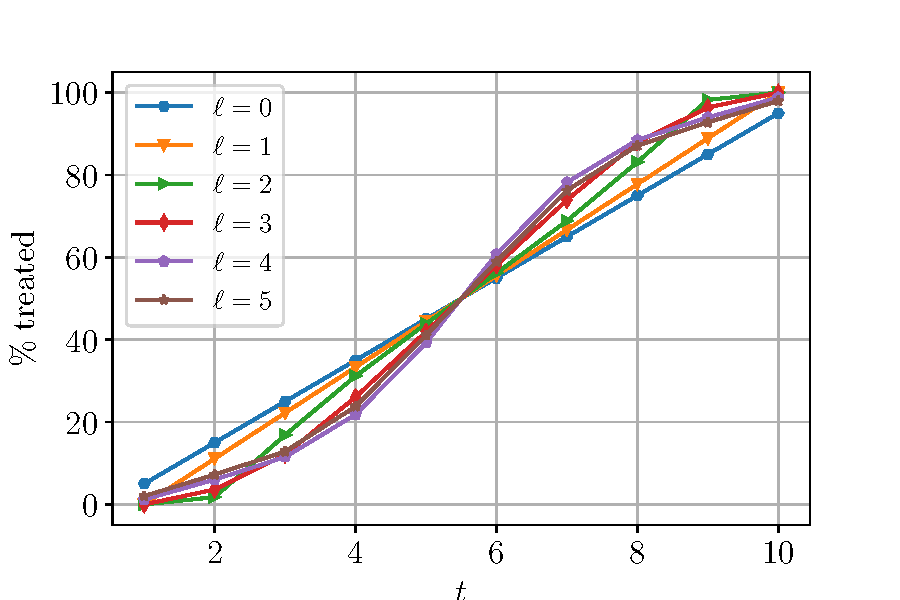
\includegraphics[width=0.5\linewidth]{plots/illustration/carryover-d-optimal.pdf}
			\caption{{D}-optimal treatment design: Optimal treated proportion ($(1+\omega_t)/2$) at each period for a $T$-period treatment design and various $\ell$, where $T = 10$. Different colors represent different $\ell$.}
			\label{fig:carryover-treatment-effect-d-opt}
		\end{figure}
		
		

\subsection{Reversible Treatment Adoption Case}\label{subsec:reversible-treatment}

There are two ways to look at the reversible treatment adoption case: first, each unit is treated at most once; second, units can be treated more than once. Surprisingly, the first case is a special case of the irreversible pattern introduced in Section \ref{sec:experiment-outcome-estimand}, as shown in \ref{subsubsec:one-time-treatment}.  For the second case, we derive analogous results as those for the irreversible pattern in \ref{subsubsec:general-reversible-treatment}.

\subsubsection{Equivalent Representation of One-time Treatment}\label{subsubsec:one-time-treatment}
\texttt{} \\
For the one-time treatment, such as the participation of a job-training or skill-improvement program, we can still use specification \eqref{eqn:model-setup} to estimate how the effect of this one-time treatment varies with the time. However, we need to use a different definition of $z_{it}$ in specification \eqref{eqn:model-setup}: $z_{it} = +1$ denotes that unit $i$ has been treated up to time $t$, and $z_{it} = -1$ denotes otherwise.

An alternative approach is to use the definition of treatment variable as in the main text: Let $w_{it} = \{0,1\}$ denote whether unit $i$ is treated at time $t$ ($w_{it} = 1$) or not ($w_{it} = 0$). In the case of one-time treatment, at most one of $w_{it}, \cdots, w_{i,t-\ell}$ is $1$. Consider the following specification using $w_{it}$:
\begin{equation}\label{eqn:model-setup-one-time}
    Y_{it}  = \tilde\alpha_i +  \tilde\beta_t + \*X_i^\T  \bm{\theta}_t + \*u_i^\T \*v_t + \tilde\tau_0 w_{it} + \tilde\tau_1 w_{i,t-1} + \cdots + \tilde\tau_{\ell} w_{i,t-\ell}  + \varepsilon_{it}\,.
\end{equation}
$\tilde\tau_j$ can be interpreted as the treatment effect given that a unit was treated $j$-period ago. If $|\tilde \tau_\ell| < \cdots < |\tilde \tau_1| < |\tilde \tau_0| $, then the effect of the one-time treatment attenuates over time.

We can show that specification \eqref{eqn:model-setup-one-time} using $w_{it}$ is equivalent to specification \eqref{eqn:model-setup} using $z_{it}$ with the change of variables:
\begin{align*}
    \tilde\tau_j = 2 \sum_{k = 0}^j \tau_k \qquad \tilde\alpha_i = \alpha_i -\sum_{k = 0}^\ell \tau_k \qquad \tilde\beta_t = \beta_t.
\end{align*}

\subsubsection{General Reversible Treatment Pattern}\label{subsubsec:general-reversible-treatment}
\texttt{} \\
Next we consider the case where a unit can arbitrarily switch between treatment and control ({\it i.e.}, Assumption \ref{ass:treatment-adoption} is violated). Below we provide the optimality conditions of T-optimal design for this case. 

\begin{proposition}\label{prop:rev-treat}
			Suppose Assumption \ref{ass:model} holds, and the treatment is reversible. Let $\omega_t =  \sum_{i = 1}^N z_{it}/N $ and $\zeta_i = \sum_{i = 1}^T z_{it} /T$.
			\begin{enumerate}
				\item Suppose $\tau$ is estimated from the least squares estimator under the specification $Y_{it} =\beta_t+ \tau z_{it} + \varepsilon_{it}$. If $\varepsilon_{it}$ is i.i.d. in $i$ and $t$ with mean $0$ and variance $\sigma_\varepsilon^2$, then any treatment design is optimal if it satisfies
				\[\omega_t = 0.\]
				\item Suppose $\tau$ is estimated from the least squares estimator under the specification $Y_{it} =\alpha_i+ \tau z_{it} + \varepsilon_{it}$. If $\varepsilon_{it}$ is i.i.d. in $i$ and $t$ with mean $0$ and variance $\sigma_\varepsilon^2$, then any treatment design is optimal if it satisfies
				\[\zeta_i = 0.\]
				\item Suppose $\tau$ is estimated from the least squares estimator under the specification $Y_{it} =\alpha_i+ \beta_t +\tau z_{it} + \varepsilon_{it}$. If $\varepsilon_{it}$ is i.i.d. in $i$ and $t$ with mean $0$ and variance $\sigma_\varepsilon^2$, then any treatment design is optimal if it satisfies
				\[\omega_t = 0, \quad \zeta_i = 0.\]
				\item Suppose $\tau$ is estimated from the least squares estimator under the specification $\alpha_i +  \beta_t +  \*X^\T_i  \bm{\theta}_t+  \*u^\T_i \*v_t + \tau_0 z_{it} + \tau_1 z_{i,t-1} + \cdots + \tau_{\ell} z_{i,t-\ell} + \varepsilon_{it}$ for $\ell \geq 0$. Suppose the assumptions in  Theorem \ref{thm:obs-latent-carryover-model} hold, and both $\*X_i$ and $\*u_i$ are discrete-valued. Let $\omega_{g,t} = \frac{1}{|\tlo_g|} \sum_{i \in \tlo_g} z_{it}$, where $\tlo_g = \{i: X_i = x_g, u_i = u_{0,g}\}$. Any treatment design is optimal if it satisfies
				\[\omega_{g,t} = 0, \, \text{ for all $t$ and $g$}, \quad \zeta_i^{(j)} = 0, \, \text{ for all $i$ and $j$},\]
    where $\zeta_i^{(j)} = \sum_{t=j}^{T - \ell+j-1} z_{it} / (T - \ell)$
			\end{enumerate}
		\end{proposition}
		
		\proof{Proof of Proposition \ref{prop:rev-treat}}
		\begin{enumerate}
		    \item Under the specification  $Y_{it} =\beta_t+ \tau z_{it} + \varepsilon_{it}$, the precision of $\hat{\tau}$ equals  
		    \[\Prec(\hat{\tau}) = NT - N \sum_{t=1}^T \omega_t^2.  \]
		    The precision is maximized at $\omega_t = 0$.
		    \item Under the specification $Y_{it}= \alpha_i + \tau z_{it} + \varepsilon_{it}$, the precision of $\hat{\tau}$ equals  
		    \[\Prec(\hat{\tau}) = NT - T \sum_{i = 1}^N \zeta_i^2. \]
		    The precision is maximized at $\zeta_i = 0$.
		    \item  Under the specification $Y_{it}= \alpha_i + \beta_t + \tau z_{it} + \varepsilon_{it}$, from the proof of Lemma \ref{lemma:simplify-obj}, the precision of $\hat{\tau}$ equals 
		    \[\Prec(\hat{\tau}) = NT - \left(T \sum_{i = 1}^{N} \zeta_i^2 -\frac{N}{T} \Lp\sum_{t=1}^T \omega_t  \Rp^2 + N \sum_{t = 1}^T \omega_t^2 \right). \]
		    The precision is maximized at $\zeta_i = 0$ and $\omega_t = 0$, given that $\sum_{t = 1}^T \omega_t^2 - \frac{1}{T}  \Lp\sum_{t=1}^T \omega_t  \Rp^2$ is minimized at $\omega_t = 0$.
		    \item Under the specification $Y_{it} = \alpha_i +  \beta_t +  \*X^\T_i  \bm{\theta}_t+  \*u^\T_i \*v_t + \tau_0 z_{it} + \tau_1 z_{i,t-1} + \cdots + \tau_{\ell} z_{i,t-\ell} + \varepsilon_{it}$, the role of observed and latent covariates in the optimal design is the same as that in Theorem \ref{thm:obs-latent-carryover-model}.   The major difference with Theorem \ref{thm:obs-latent-carryover-model} is the optimal treated fraction conditions. Note that the precision matrix $\Prec(\hat{\bm{\tau}})$ takes the form of (see Equation \eqref{eqn:precision-matrix}), 
      \[\Prec\left( \hat{\bm{\tau}}\right) =  \bm{Z}_\ell^\T  \bm{\Sigma}^\I_e  ( \bm{\Sigma}_e - \bm{\Gamma} (\bm{\Gamma}^\T \bm{\Sigma}^\I_e  \bm{\Gamma})^\I \bm{\Gamma}^\T) \bm{\Sigma}^\I_e  \bm{Z}_\ell  \]
where the $(j,j)$-th entry ({\it i.e.}, diagonal entry) in $\Prec\left( \hat{\bm{\tau}}\right)$ takes the form of (see Equations \eqref{eqn:precision-entries-1} and \eqref{eqn:precision-entries-2} in Lemma \ref{eqn:carryover-separate-obj}, and the proof of Lemma \ref{lemma:simplify-obj})
\begin{align*}
    & N(T-\ell) -   \Bigg[  N \sum_{t=j}^{T - \ell+j-1} \omega_t^2   - \frac{N}{T - \ell}  \Lp \sum_{t=j}^{T - \ell+j-1} \omega_t  \Rp^2    + (T - \ell) \sum_{i = 1}^N (\zeta_i^{(j)})^2 \Bigg] \\ & - \frac{N}{\sigma_\varepsilon^2} \sum_{j = 1}^{\ell + 1} f_{j,\*X}(Z) - \frac{N}{\sigma_\varepsilon^2} \sum_{j = 1}^{\ell + 1} f_{j,\*U}(Z)
\end{align*}
$f_{j,\*X}(Z)$ and $f_{j,\*U}(Z)$ are defined in Lemma \ref{lemma:simplify-obj}.
The $(j,j)$-th entry in $\Prec(\hat{\bm{\tau}})$ is maximized at $\omega_t = 0$ for all $t$ and $\zeta_i^{(j)} = 0$ for all $i$. Moreover both $f_{j,\*X}(Z)$ and $f_{j,\*U}(Z)$ are minimized at $\omega_{g,t} = 0$. The T-optimal design maximizes the trace of the precision matrix, which is satisfied by the solution provided in Lemma \ref{prop:rev-treat}.4. 
		\end{enumerate}
		We conclude the proof of Lemma \ref{prop:rev-treat}. \Halmos
		\endproof
		
		
		    \subsection{A Rounding Approach for A Feasible Solution}\label{subsubsec:practical-considerations}
    
    When there does not exist a feasible solution in $\mathbb{A}^{\mathrm{disc}}_{\mathrm{opt}}$,  we suggest using the nearest integer rounding rule as follows to obtain a feasible $\{A_i\}_{i \in [N]}$. 
    
	
	\textit{Nearest integer rounding rule:} If the number of treated units for each stratum suggested by Theorem \ref{thm:obs-latent-carryover-model}, {\it i.e.}, is not an integer,
 \[\frac{|\tlo_g|(1+\omega_{\ell,t}^\ast)}{2T}\]
  we suggest rounding it to an integer using the nearest integer rule. We separate the number of treated units into the integer and decimal parts
 \[\frac{|\tlo_g|(1+\omega_{\ell,t}^\ast)}{2T} = \underbrace{\lfloor \frac{|\tlo_g|(1+\omega_{\ell,t}^\ast)}{2T} \rfloor }_{N_{\mathrm{treated},g,t}^{\mathrm{int}}} + \underbrace{\frac{|\tlo_g|(1+\omega_{\ell,t}^\ast)}{2T} - \lfloor \frac{|\tlo_g|(1+\omega_{\ell,t}^\ast)}{2T} \rfloor }_{N_{\mathrm{treated},g,t}^{\mathrm{dec}}} \]
 The nearest integer rounding rule works as follows
\begin{itemize}
    \item If the decimal part $N_{\mathrm{treated},g,t}^{\mathrm{dec}} < 0.5$, or if $N_{\mathrm{treated},g,t}^{\mathrm{dec}} = 0.5$ with $t < T/2$, then the rounded number of treated units is 
    \[\frac{1}{|\tlo_g|} \sum_{i \in \tlo_g} \boldsymbol{1}_{A^\rnd_i \leq t} = N_{\mathrm{treated},g,t}^{\mathrm{int}}  \]
    \item Otherwise, the rounded number of treated units is
    \[\frac{1}{|\tlo_g|} \sum_{i \in \tlo_g} \boldsymbol{1}_{A^\rnd_i \leq t} = N_{\mathrm{treated},g,t}^{\mathrm{int}} + 1  \]
\end{itemize}

Let $Z^\rnd$ be the treatment design satisfying the rounded number of treated units for each stratum. Let $Z^{\mathrm{int}\ast}$ be the optimal integer solution to optimization problem \eqref{eqn:obj}. $ \tr \big(\mathrm{Prec}(\hat{\bm{\tau}})  \big)_{Z} $ be the objective function \eqref{eqn:obj} ({\it i.e.} $\tr \big(\mathrm{Prec}(\hat{\bm{\tau}})  \big)$) evaluated at $Z$.
 
	The following proposition bounds the difference between $ \tr \big(\mathrm{Prec}(\hat{\bm{\tau}})  \big)_{Z^\rnd} $ and $ \tr \big(\mathrm{Prec}(\hat{\bm{\tau}})  \big)_{Z^{\mathrm{int}^\ast}} $.
	\begin{proposition}
		\label{prop:rounding-error-obs-cov}
		Suppose the assumptions in Theorem \ref{thm:obs-latent-carryover-model} hold, $d_u = 0$ and $N$ is even, and $x_{k,\max} = \max_{g} |x_{gk}|$ is finite, where $x_{gk}$ is the $k$-th coordinate of $x_g$ for all strata $g$. We have
		\[ \tr \big(\mathrm{Prec}(\hat{\bm{\tau}})  \big)_{Z^\rnd} = \tr \big(\mathrm{Prec}(\hat{\bm{\tau}})  \big)_{Z^{\mathrm{int}\ast}}  \cdot\left(1+ O\left(\frac{1+ \sum_{k=1}^{d_x} x_{k,\max}^2}{N^2_{\min}} \right) \right).\]
	\end{proposition}


    Since the probability of each realization of $\*X_i$ is bounded away from 0 and $x_{k,\max}$ is finite,  we have $O\left((1+ \sum_{k=1}^{d_x} x_{k,\max}^2)/N^2_{\min} \right)  = O \Lp 1/N^2 \Rp$ as $N \rightarrow \infty$. However, if $G$ is large compared with $N$ (or $\*X_i$ takes infinitely many values), $ \tr \big(\mathrm{Prec}(\hat{\bm{\tau}})  \big)_{Z^\rnd} $ could be much larger than $ \tr \big(\mathrm{Prec}(\hat{\bm{\tau}})  \big)_{Z^{\mathrm{int}\ast}} $. In this case, we could instead partition units into only a few ({\it e.g.}, 2 or 3) groups based on their covariates' values using $K$-means or some other methods. Within each group, the treated fraction conditions are satisfied. 
    
    {\blue 
    \subsection{Supplementary Details in Choosing a Treatment Design}\label{subsec:more-details-choose-design}
    
    In Algorithm \ref{algo:choose-design}, we provide a procedure to randomly choose a treatment design for each stratum based on the treated fraction conditions. If there are no covariates (in the outcome model), then this is the case where we only have one stratum that consists of all experimental units. 
    
    We want to highlight that Algorithm \ref{algo:choose-design} allows for the case where the treatment fraction conditions in Theorem \ref{thm:obs-latent-carryover-model} can not be exactly satisfied for any treatment design. For this case, Algorithm \ref{algo:choose-design} uses the nearest integer rounding algorithm in \ref{subsubsec:practical-considerations} in choosing a treatment design.
    
    
    	\begin{algorithm}[htp]
 \caption{Choose a treatment design for each stratum $g$}  \label{algo:choose-design}
 \SetKwInOut{Input}{Inputs}
 \nl \Input{$|\mathcal{O}_g|$, $[\omega_{\ell,t}^\ast]_{t\in [T]}$} 
  \nl \For{$t = 1,\cdots, T $}{
  \nl $N_{\mathrm{treated},g,t}^{\mathrm{int}} \leftarrow \lfloor |\tlo_g|(1+\omega_{\ell,t}^\ast)/2 \rfloor$\;
  \nl $N_{\mathrm{treated},g,t}^{\mathrm{dec}} \leftarrow |\tlo_g|(1+\omega_{\ell,t}^\ast)/2-  N_{\mathrm{treated},g,t}^{\mathrm{int}} $ \;
  \nl \eIf{$N_{\mathrm{treated},g,t}^{\mathrm{dec}} < 0.5 $ or $ N_{\mathrm{treated},g,t}^{\mathrm{dec}} = 0.5 $ with $t < T/2$}{
  \nl $N_{g,t} \leftarrow N_{\mathrm{treated},g,t}^{\mathrm{int}} $ \;}{
  \nl $N_{g,t} \leftarrow N_{\mathrm{treated},g,t}^{\mathrm{int}} + 1 $ \;
  } 
    }
  \nl $f(\cdot)  \leftarrow $ a random function that shuffles $\{1, 2, \cdots, |\mathcal{O}_g| \}$\;
  \nl $Z_g \leftarrow [-1]^{|\mathcal{O}_g| \times T}$ \;
  \nl \For{$i = 1, \cdots, |\mathcal{O}_g|$}{
  \nl \For{$t = 1, \cdots, T$}{
  \nl \eIf{$f(i) \leq N_{g,t}$}{
  $z_{g,it} \leftarrow 1$ \;
  }{
  $z_{g,it} = -1$ \;
  }
  }
  }
  \nl \KwRet $Z_g $\;
\end{algorithm} 
    

\subsection{Latent Covariates}\label{subsec:latent-covariates}

\subsubsection{Estimation of latent covariates}\label{subsubsec:estimate-latent-covariates}
\texttt{}
 
If there are latent covariates, we suggest, whenever possible, using the historical control data for the same set of units in designing the experiment. This is because historical data has information about $\*u_i$. Below we provide a heuristic approach to using historical data to find a better treatment design. 


We can apply singular value decomposition (SVD) to the historical data and take the top singular vectors as the estimated $\*u_i$, denoted as $\hat{\*u}_i$. We can use cross-validation to choose the number of singular vectors.
Specifically, we can partition the historical data in the time dimension into training and validation sets. Then we estimate the singular vectors on the training set, and design synthetic experiments on the validation set based on various numbers of singular vectors. Finally, we can select the optimal number of singular vectors whose experimental design has the lowest estimation error of treatment effects on the validation set.

We suggest using SVD with cross-validation for the following reason. Since the time horizon $T$ of the experiment is typically short ({\it e.g.}, one flu season with $T = 7$ in our empirical application, and short $T$ is the regime where statistical power is a concern), it is typically sufficient to account for the first one or two latent factors in the feasible GLS estimator. Then it is natural to account for the top a few latent factors in the design of experiments, where SVD with cross-validation seems to be a reasonable approach. 

If historical data have missing observations, or if both the historical data and experimental data have a long time horizon (where it is reasonable to estimate more latent factors), then we could use low-rank matrix estimation with nuclear norm regularization to estimate latent covariates from the historical data.


\subsubsection{Non-adaptive treatment design based on latent covariates}\label{subsubsec:choose-treatment-design}
\texttt{}

We can first estimate latent covariates by SVD from historical data, and then treat $\hat{\*u}_i$ as ``observed'' covariates in the design of non-adaptive experiments. If $\hat{\*u}_i$ is continuous, then we can partition units into strata based on $\hat{\*u}_i$ by applying $k$-means clustering on the largest singular vectors, similar to observed continuous-valued covariates. Here the number of clusters $k$ can be chosen by cross-validation. Each cluster of units from $k$-means clustering is a stratum, and we can apply Algorithm \ref{algo:choose-design} to randomly choose a treatment design for each stratum. 

The approach of stratifying based on top singular vectors is conceptually similar to spectral clustering, which enjoys nice theoretical and empirical properties (see {\it e.g.}, \cite{ng2001spectral}) and works well in our empirical applications. Admittedly, it is possible to stratify based on the ideas of other clustering algorithms ({\it e.g.}, density-based clustering, mean-shift clustering), and we leave this for future work. 


Note that it seems possible to use the currently available experimental data to improve the estimation precision of $\hat{\*u}_i$ and treatment decisions for subsequent experimental periods. However, we do not pursue this route for two reasons.

First, if historical data does not have many periods, then $\hat{\*u}_i$ can be quite noisy early in the experiment. We may not want to use noisy estimates of $\*u_i$ for treatment decisions, because the mistakes we make in the early periods (due to very noisy estimates of $\*u_i$) can carry over to later periods. We have verified this in numerical simulations but did not include them in the paper, given the paper is quite lengthy already.

Second, if historical data has many periods, which allows us to precisely estimate $\*u_i$, then having a few more experimental periods can only marginally improve the precision of $\hat{\*u}_i$ and treatment allocations. This is because the convergence rate of $\hat{\*u}_i$ is $\sqrt{T}$ \citep{bai2003inferential}.





    \subsection{Separable Quadratic Representation}\label{subsec:separate-quadratic}
    
    In this subsection, we state a critical lemma that shows $\tr\left(\mathrm{Prec}(\hat{\bm{\tau}})\right) $ can be decomposed into three separable quadratic functions: the first one does not depend on $\*X$ and $\*U$, the second one only depends on $\*X$, and the third one only depends on $\*U$. The solutions to each of these three show the effects of fixed effects, observed covariates, and latent covariates on the optimal treatment assignments, respectively. If a solution simultaneously optimizes all three quadratic functions, then this solution is an optimal solution to \eqref{eqn:obj}.
    
    \begin{lemma}[Separable Quadratic Representation]\label{lemma:simplify-obj}
		Suppose Assumptions \ref{ass:treatment-adoption}, \ref{ass:model}, and \ref{ass:constant-error} hold. Suppose $\hat{\bm{\tau}} $ is estimated from the infeasible GLS with $\*W= [w_{ij}] \propto \big(\*U \*\Sigma_v \*U^\T + \sigma_\varepsilon^2 \*I_N \big)^\I $,  rows in $\*X$ and $\*U$ are demeaned, that is, $\sum_{i = 1}^N \*X_i = \bm{0}_{d_x}$ and $\sum_{i = 1}^N \*u_i = \bm{0}_{d_u}$,  $\sum_{i = 1}^N \*X_i \*u_i^\T = \mathbf{0}_{d_x,d_u}$, and $\*\Sigma_v = \sigma_\varepsilon^2 \cdot \*I_{d_u}$.
		Let $T_\ell = T - \ell$ and $j_\ell = j + T_\ell - 1$ for all $j$. Then $\tr \big(\mathrm{Prec}(\hat{\bm{\tau}})  \big) $  takes the form of
		\begin{equation}\label{eqn:carryover-quadratic}
		\begin{aligned}
		\tr \big(\mathrm{Prec}(\hat{\bm{\tau}})  \big)  =& - \frac{N}{\sigma_{\varepsilon}^2} \sum_{j = 1}^{\ell+1} 
		\bigg(  \underbrace{ (\bm{\omega}_{j:j_\ell})^\T \*P_{\bm{1}_{T_\ell}}  \bm{\omega}_{j:j_\ell}  + 2 \bm{b}_{\ell}^\T \bm{\omega}_{j:j_\ell} }_{f_{j,\bm{1}}(Z)} +  \underbrace{\textstyle  \sum_{k=1}^{d_x}  (\bm{\omega}_{j:j_\ell}^{x_k})^\T \*P_{\bm{1}_{T_\ell}}  \bm{\omega}_{j:j_\ell}^{x_k}  }_{f_{j,\*X}(Z)} + \underbrace{\textstyle \frac{1}{N} \bm{z}_{j:j_\ell}^\T \*M_{\*U} \bm{z}_{j:j_\ell} }_{f_{j,\*U}(Z)} \bigg),
		\end{aligned}
		\end{equation}
		where $\bm{\omega}_{j:j_\ell} = \big({\omega}_j, \cdots, {\omega}_{j_\ell}\big)^\T$ with ${\omega}_t = \frac{1}{N} \sum_{i=1}^N z_{it} $, $\bm{\omega}_{j:j_\ell}^{x_k} = \big(	{\omega}^{x_k}_j, \cdots, {\omega}^{x_k}_{j_\ell} \big)^\T$ with ${\omega}^{x_k}_t =\frac{1}{N} \sum_{i=1}^N X_{ik} z_{it}$, 
		$\bm{z}_{j:j_\ell} = \big(\*z_{j}^\T, \cdots, \*z_{j_\ell}^\T \big)^\T \in \{-1,+1\}^{N T_\ell\times 1}$,  $\*P_{\bm{1}_{T_\ell}} = \*I_{T_\ell} - \frac{1}{T_\ell} \bm{1}_{T_\ell} \bm{1}_{T_\ell}^\T$, $\*b_\ell = [b_{\ell,t}] \in [-1,1]^{T_\ell}$ with $b_{\ell,t} = \frac{T_\ell+2-2t}{T_\ell} $, and $\*M_{\*U} = \*P_{\bm{1}_{T_\ell}} \otimes \*U (\*I_{d_u} + \*U^\T \*U)^\I \*U^\T$.\footnote{``$\otimes$'' is the Kronecker product.}
	\end{lemma}

    
    From Lemma \ref{lemma:simplify-obj}, maximizing $	\tr \big(\mathrm{Prec}(\hat{\bm{\tau}})  \big)$ is equivalent to 
	\begin{equation}\label{eqn:objective-reduced}
	 \min_{\{A_i\}_{i \in [N]} }  \underbrace{\textstyle \sum_{j = 1}^{\ell+1}   f_{j,\bm{1}}(Z)  }_{f_{\bm{1}}(Z) }  + \underbrace{\textstyle \sum_{j = 1}^{\ell+1}   f_{j,\*X}(Z) }_{f_{\*X}(Z) }  + \underbrace{\textstyle \sum_{j = 1}^{\ell+1}   f_{j,\*U}(Z)  }_{f_{\*U}(Z) }. 
	\end{equation}

    If we can find an $\{A_i\}_{i \in [N]}$ that simultaneously minimizes each of $f_{\bm{1}}(Z)$, $f_{\*X}(Z)$, and $f_{\*U}(Z)$, then this $\{A_i\}_{i \in [N]}$ minimizes \eqref{eqn:objective-reduced}. In the following, we separately analyze the three sub-problems of \eqref{eqn:objective-reduced}: $\min_{\{A_i\}_{i \in [N]} }  f_{\bm{1}}(Z) $, $\min_{\{A_i\}_{i \in [N]} }  f_{\*X}(Z) $, and $\min_{\{A_i\}_{i \in [N]} }  f_{\*U}(Z) $.

	We first consider the sub-problem $\min_{\{A_i\}_{i \in [N]} }  f_{\bm{1}}(Z) $. The solution to this problem characterizes the effect of the presence of two-way fixed effects, $\alpha_i$ and $\beta_t$ on the optimal treatment assignments. Note that $f_{\bm{1}}(Z)$ is a sum of quadratic and linear terms:
	\begin{equation}\label{eqn:f1w-carryover-obj}
	   f_{\bm{1}}(Z) =\sum_{j = 1}^{\ell+1} \big( (\bm{\omega}_{j:j_\ell})^\T \*P_{\bm{1}_{T_\ell}}  \bm{\omega}_{j:j_\ell}  + 2 \bm{b}_{\ell}^\T \bm{\omega}_{j:j_\ell} \big).
	\end{equation}
	It is possible to provide the analytical solution to $\min_{\{A_i\}_{i \in [N]} }  f_{\bm{1}}(Z) $ based on its first order condition. The analytical solution is provided in \eqref{eqn:omega-carryover}. 
	
	
	Next we consider the other two sub-problems: $\min_{\{A_i\}_{i \in [N]} }  f_{\*X}(Z) $ and $\min_{\{A_i\}_{i \in [N]} }  f_{\*U}(Z) $. The solution to these two problems characterizes the effects of the presence of $\*X_i$ and/or $\*u_i$ on the optimal treatment assignments, respectively. 
	Note that both $f_{\*X}(Z) $ and $f_{\*U}(Z) $ are sums of quadratic functions of $\{\*z_t\}_{t=1}^T$ that do not have linear terms. The Hessian of $f_{\*X}(Z) $ and $f_{\*U}(Z) $ are both semidefinite, following the definition of two matrices in $f_{\*X}(Z) $ and $f_{\*U}(Z) $, {\it i.e.}, $\*P_{\bm{1}_{T_\ell}} = \*I_{T_\ell} - \frac{1}{T_\ell} \bm{1}_{T_\ell} \bm{1}_{T_\ell}^\T$ and $\*M_{\*U} = \*P_{\bm{1}_{T_\ell}} \otimes \*U (\*I_{d_u} +  \*U^\T \*U)^\I \*U^\T$. Then the minimum possible value of $f_{\*X}(Z) $ and $f_{\*U}(Z) $ is 0. As shown in Theorem \ref{thm:obs-latent-carryover-model} below, the minimum value of $f_{\*X}(Z) $ can be achieved if $\{A_i\}_{i \in [N]} \in \mathbb{A}_{\*X}$, and the minimum value of $f_{\*U}(Z)$ can be achieved if $\{A_i\}_{i \in [N]} \in \mathbb{A}_{\*U}$.

}

\clearpage


